% To learn more - Search `beamer-template` or see this https://www.overleaf.com/learn/latex/Beamer

\documentclass{beamer}
\usepackage[utf8]{inputenc}

\usetheme{Madrid}
\usecolortheme{default}

%------------------------------------------------------------
%This block of code defines the information to appear in the
%Title page
\title[Threshold Based \textit{K}-Means Monitoring] %optional
{Continuous k-Means Monitoring
over Moving Objects}

\subtitle{A Threshold Based Approach}

\author[Group 7] % (optional)
{Aasneh Prasad \and Gautam Sharma \and Pranav Jain \and Sahil Danayak \and Sreehari \and Dhanesh}


\date[16th November 2023] % (optional)
{\textbf{DA321M Course Project, July-Nov 2023}}

\logo{
\includegraphics[height=1cm]{iitg-logo.jpeg}}

%End of title page configuration block
%------------------------------------------------------------



%------------------------------------------------------------
%The next block of commands puts the table of contents at the 
%beginning of each section and highlights the current section:

\AtBeginSection[]
{
  \begin{frame}
    \frametitle{Table of Contents}
    \tableofcontents[currentsection]
  \end{frame}
}
%------------------------------------------------------------


\begin{document}

%The next statement creates the title page.
\frame{\titlepage}


%---------------------------------------------------------
%This block of code is for the table of contents after
%the title page
\begin{frame}
  \frametitle{Table of Contents}
  \tableofcontents
\end{frame}
%---------------------------------------------------------


%---------------------------------------------------------
\section{HC* Algorithm}
\begin{frame}
  \frametitle{HC* Algorithm}

  \begin{columns}

    \column{0.45\textwidth}
    \begin{itemize}
      \item Uses data from the previous iterations to form new clusters.
      \item  It exploits the fact that only points close to the perpendicular bisectors defined by the centers, may change clusters.
      \item Less computationally expensive
      \item $P_{active}$ of points whose clusters have been reassigned.

    \end{itemize}

    \column{0.5\textwidth}
    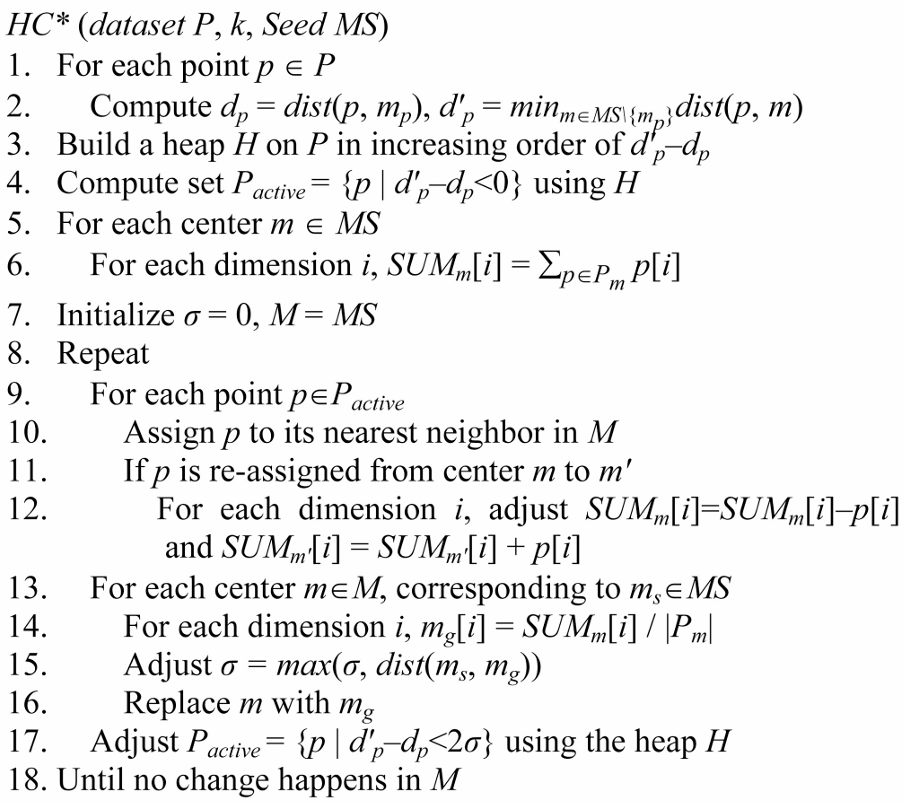
\includegraphics[width=1\textwidth]{Pic1.png}

  \end{columns}
\end{frame}

%---------------------------------------------------------
\section{Assignment of thresholds}
\begin{frame}
  \frametitle{Assignment of thresholds}
  The threshold assignment routine takes as input the
  objects locations \(P = \{p1, p2, \ldots, pn\}\) and the k-means set
  \(\{m1, m2, \ldots, mk\}\), and outputs a set of \(n\) real values \(\{\theta 1, \theta 2, \ldots, \theta n\}\), i.e., the thresholds.
  \begin{itemize}
    \item It can be derived that \[ \theta_p \leq \min_{m \in M \setminus \{m_p\}} \text{dist}(p, m) - \triangle \], where $\triangle$ represents the maximum permissible error.
          \vspace{5mm}
    \item Based on the following observation we can develop an algorithm as given below for calculating the thresholds or maximum distance each object can move without sending a signal to the server in its neighbourhood
  \end{itemize}


\end{frame}


\begin{frame}
  \frametitle{Algorithm for calculating thresholds}


  \begin{center}
    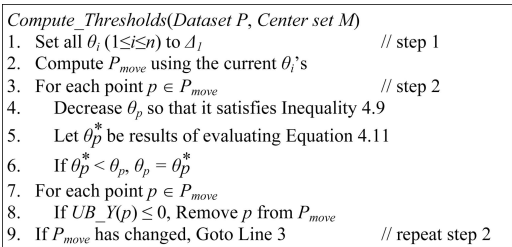
\includegraphics[width=\textwidth]{algo.png} % Replace with the actual file name

  \end{center}
\end{frame}
%------------------------------------------------------------

%---------------------------------------------------------
\section{Utilizing Object Speed and Dissemination of Thresholds}
\begin{frame}
  \frametitle{Utilizing Object Speed and Dissemination of Thresholds}
  Assume the system knows roughly the average speed $s_{i}$ of each object $p_{i}$, then the objective function becomes $\sum\limits_{i=1}^n s_i/\theta_i$.
  \begin{itemize}
    \item Optimal solution using Lagrange multiplier: $\forall i,\space \theta_{i} = (n\triangle_{1} \sqrt{s_{i}})/(\sum\limits_{j=1}^n \sqrt{s_{j}})$
    \item Dissemination of Thresholds can be carried out depending on the computational capabilities of the objects. We propose two approaches:
          \begin{itemize}
            \item The first is
                  based on broadcasting. Initially, the
                  server broadcasts $\triangle$. Then each object
                  computes its own threshold based on the broadcast
                  information.
            \item The second approach assumes that objects have limited
                  computational capabilities. Initially, the server sends $\triangle_{1}$ to
                  all objects through single-cast messages. In subsequent
                  updates, it sends the threshold to an object only when it has
                  changed.
          \end{itemize}
  \end{itemize}


\end{frame}



%---------------------------------------------------------
\section{Experimental Evaluation}
\begin{frame}
  \frametitle{Comparision of CPU Time}

  \begin{columns}

    \column{0.35\textwidth}
    \begin{itemize}
      \item This graph shows the comparison of CPU times of \texttt{REF} (Normal K-means algorithm) v/s \texttt{TKM} (Threshold-based K-Means algorithm)
      \item At each iteration, some new points were added and, with a probability, the previous points were displaced by a small amount.


    \end{itemize}

    \column{0.65\textwidth}
    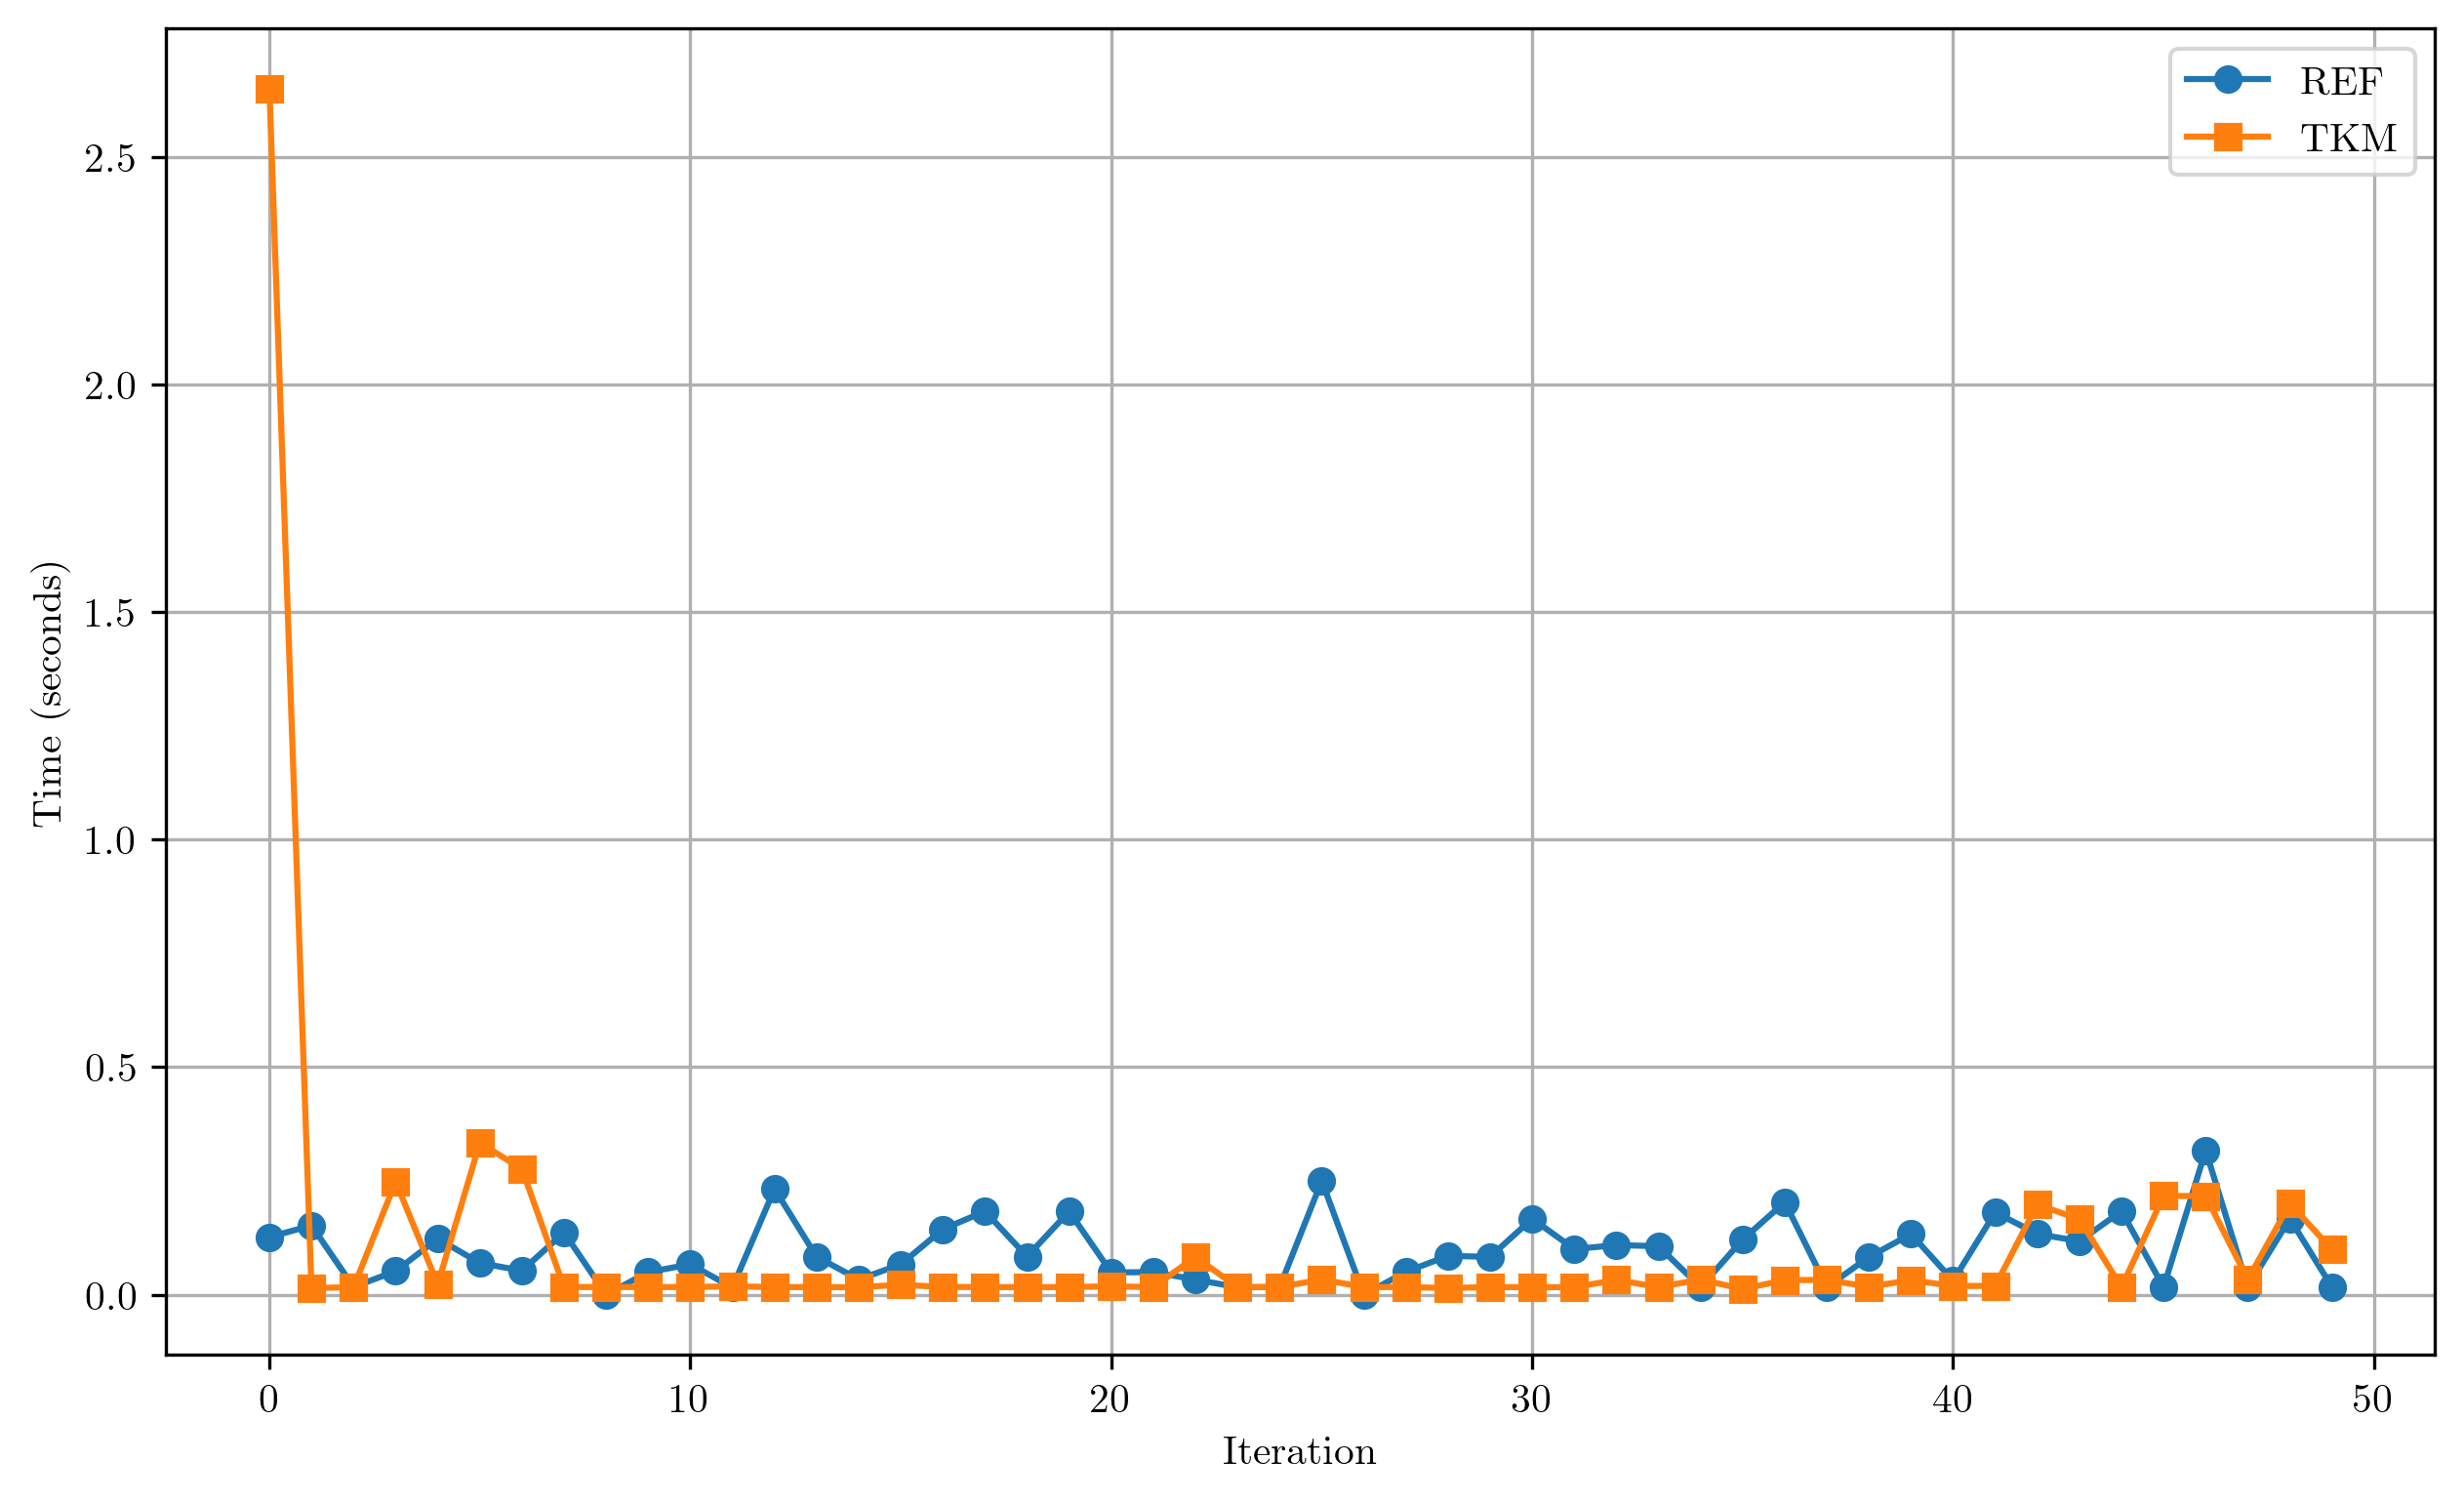
\includegraphics[width=1\textwidth]{Diff.png}
    \begin{itemize}
      \vspace{-0.2cm}
      \item \small This graph shows \texttt{TKM} performs much better in most of the cases.
    \end{itemize}
  \end{columns}
\end{frame}
%---------------------------------------------------------



\end{document}
